\documentclass[serif,9pt,xcolor=dvipsnames]{beamer}
\usetheme{default}

%\usepackage[english]{babel}    % deutsche Sonderzeichen, Trennmuster, etc
\usepackage[german]{babel}    % deutsche Sonderzeichen, Trennmuster, etc

\usepackage[T1]{fontenc} 
\usepackage[utf8]{inputenc}  % deutsche Umlaute


\usetheme[]{Warsaw}
%\usetheme[]{Rochester}

%  \usecolortheme[named=Brown]{structure} 
%\usecolortheme[]{crane} 
%\usecolortheme[]{rose} 
\usecolortheme[]{christian1} 

% Mathekram
%\usepackage{amsmath}
%\usepackage{amsfonts}
%\usepackage{amssymb}

% Graphiken
%\usepackage{epsfig}            % Paket zum Einbinden von postscript Graphiken
\usepackage{graphicx}		% Andere Graphikdateien einbinden
\usepackage{float}             % Hilfesmakros beim Positionieren von Graphiken
\usepackage{color}
%\usepackage{subfig}
\usepackage{textcomp}


\usepackage[sc]{mathpazo}	%FONT


\usepackage{listings}


%% GLEGRAPHICS
\graphicspath{{./bilder/gleplots/}}

\newcommand{\includeglegraphics}[1]{  
%\includegraphics[]{#1.pdf}
\input{#1.inc}   
}

\newcommand{\Th}{\vartheta}

%\newcommand{\Th}{\vartheta}


\definecolor{feedforwardpath}{rgb}{0.0,1,0.0}
\definecolor{feedbackpath}{rgb}{1.0,0.0,0.0}

\DeclareRobustCommand{\vec}[1]{{\mbox{\mathversion{bold}\ensuremath{#1}}}}
\DeclareRobustCommand{\mat}[1]{{\mbox{\mathversion{bold}\ensuremath{#1}}}}

\title[]{ORTD --- The Open Realtime Dynamics Toolbox}
	\subtitle{} %Mehrgrößenregelung einer Neuro-Prothese zur Generierung von Bewegungen  der oberen Extremität mittels Neuromuskulärer Elektrostimulation (NMES)
\date{2011}
\author{Christian Klauer$^{1}$\\
{\tiny $^{1}$Fachgebiet Regelungssysteme, Technische Universität Berlin\\
Kontakt: klauer@control.tu-berlin.de}
}




\begin{document}
% \frame[plain]{\titlepage}

\author{Christian Klauer$^{1}$}

\begin{frame}
 \frametitle{Motivation und Ziele}

% \begin{tabular}{rr}
% \hspace{8cm} & \includegraphics[width=0.2\textwidth]{logo_mundus.png} 
% \end{tabular}





\end{frame}

\begin{frame}

 \frametitle{General Overview}



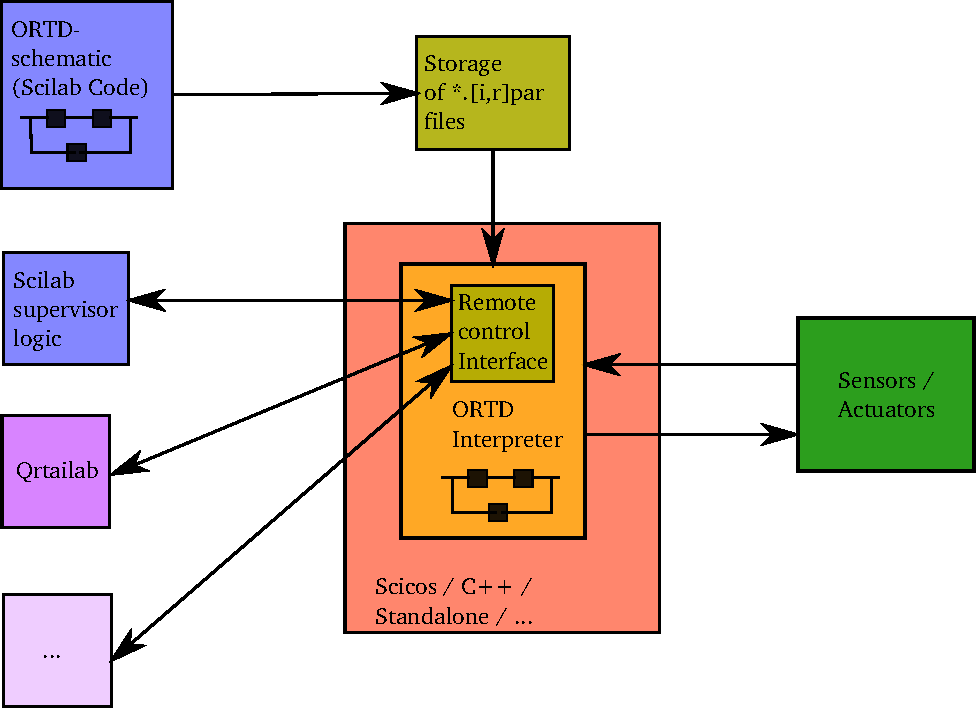
\includegraphics[trim=0mm 0mm 0mm 0mm, clip,width=0.95\linewidth]{../pictures/ortd_principle.pdf}

\end{frame}



\begin{frame}

 \frametitle{One first example}


  \begin{block}{Add Ofset Macro}

dfs

    



  \end{block}

% \begin{verbatim}
% function [sim,y] = ld\_add_ofs(sim, events, u, ofs)
%   [sim,ofs\_const] = libdyn\_new\_blk\_const(sim, events, ofs);
%   
%   [sim,y] = ld\_sum(sim, events, list(u,0, ofs\_const,0), 1,1);
% endfunction
% \end{verbatim}


% \begin{lstlisting}
% for i:=maxint to 0 do
% begin
% j:=square(root(i));
% end;
% \end{lstlisting}
% 


\end{frame}


% \frametitle{Elektrische Stimulation und Gewichtsentlastung}
% 
% \begin{block}{Prinzip}
%   \begin{itemize}
%   \item Muskeln werden elektrisch stimuliert. $\rightarrow$ Auftreten von Bewegungen
%   \item Ein Exoskelett verringert die Schwerkraft des Arms. $\rightarrow$ Es ist weniger Strom notwendig.
%   \end{itemize}
% \end{block}
% 
% 
% 
% 	\begin{columns}[c]
% 		\column[c]{4cm}
%  
%     \includegraphics[trim=0mm 0mm 0mm 0mm, clip,
%     width=0.95\linewidth]{bilder/exo.png}
%     
%     Exoskelett, TU Wien
% 
% 		\column{5cm}
% 
%     \includegraphics[trim=0mm 0mm 0mm 0mm, clip,
%     width=0.95\linewidth]{bilder/deltoid.pdf}
% %     Elektrische Stimulation der Schultermuskulatur
% 
% \end{columns}
% 
% 
% 
% \end{frame}
% 
% 
% 
% \begin{frame}
%   \frametitle{Funktionsweise des Systems}
% 
% \begin{block}{Ziel}
% \begin{itemize}
%  \item Einstellung einer Sollposition für die Hand.
%  \item Bspw. Bewegen eines Objektes vom Tisch zum Mund.
% \end{itemize}
% \end{block}
% 
% 
% 	\begin{columns}[c]
% 		\column[c]{8cm}
% 
% 
% 
% 
%   \begin{figure}[!htb]
%   \centering
%   \includegraphics[trim=00mm 140mm 00mm 00mm, clip, width=1.0\linewidth]{bilder/system_overview.pdf}
%    % \caption{Versuchsaufbau}
%   \label{fig:}
%   \end{figure}
% 
% 
% 
% 		\column{3.5cm}
% 
% \begin{block}{Funktionsweise}
%   \begin{itemize}
%    \item Messung der Arm-Winkel
%    \item Regelung reagiert auf Positionsabweichungen
%    \item Stimulation wird angepasst
%   \end{itemize}
% \end{block}
%    
% 
% 
% \end{columns}
% 
% 
% \end{frame}
% 


\end{document}
